\chapter{Design and Tools}
The design and tools that address the requirements of human biomechanics and movement analysis are examined in this chapter. The prerequisites and criteria are firstly examined to replicate the rehabilitation scenario. An in depth analysis of the Dynamic Arm Simulator (DAS) and Open Sim CMC is done to understand their possible potential. The Hill-Based Muscle Modeling technique is investigated alongside with the different DAS functionalities, emphasizing the critical role of its underlying dynamics in shaping the Model Design.

%Briefly introduce the purpose of the chapter and its significance in the context of your overall work.
%Provide an overview of the topics you will cover: investigating needs, researching information on Dynamic Arm Simulator (DAS) and Open Sim CMC, Hill-Based Muscle Modeling, DAS functionalities, and Dynamics of DAS.
\section{Criteria Analysis}

To pinpoint the crucial factors that would direct our choice of design and tools, a thorough criterion analysis was carried out. The following important standards came to be recognized as essential elements in the search for an efficient simulation solution:

\begin{enumerate}
    \item \textbf{Real Arm Simulator} In order to correctly reproduce real-world dynamics and movements, an exact simulation of an arm was required.
    \item \textbf{Accurate Dynamics Representation} To ensure that the simulated arm's behavior and responses adhere to the fundamentals of human biomechanics.
    \item \textbf{Neural Stimulation Control} An essential criteria to provide more realistic interaction between the simulated arm and the brain or the FES.
    \item \textbf{Tracking} Ability to track the arm´s movement either in joint space or task space. This will provide flexibility in the control system.
    \item \textbf{EMG Reading} It should present the capability or a possibility to read real or fake neural excitation data. This data will be used as the main driven input to control the arm's stimulation.
    \item \textbf{Control Model Integration} A key criterion is that the tool presents the possibility to develop and evaluate various control methods.
    \item \textbf{External Forces Addition} In order to simulate realistic interactions and enabling more thorough and accurate simulation of arm dynamics.
    
\end{enumerate}



\section{Dynamic Arm Simulator (DAS)}
Detail the sources you consulted during your research.
Explain why you chose Dynamic Arm Simulator
Provide an overview of Dynamic Arm Simulator and its role in your project.
Explain the key features and functionalities of DAS.
Discuss the benefits of using DAS in your design.


\subsection{Hill-Based Muscle Modelling}
Describe the Hill-Based Muscle Modeling method and its significance in biomechanics.
Explain how it is utilized within Dynamic Arm Simulator.
Discuss any advantages or limitations of this modeling approach.

\subsection{DAS Functionalities}
The Dynamic Arm Simulator (DAS) is a Matlab Mex function that contains the system dynamics and other functions, accessible via a Matlab function interface. In the following section the most relevant functions for this project are presented. 

The DAS can be downloaded from the simTK.org website (\href{https://simtk.org/projects/das}{https://simtk.org/projects/das}). It includes the \textbf{main mex file}, some coding to test the correct functionality and installation of the simulation environment and some basic manual for understanding its different capabilities. 
\subsubsection{Loading the model}

During the initialization the MEX functions reads in the parameters from the model. When initializing the model the 13 joints and 138 muscle elements are loaded.

% The model presents 298 states. It consists of 11 (one for each degree of freedom) general coordinates (rad), 11 generalized velocities (rad/s), 138 muscle contractile element (CE) lengths (relative to LCE optimal), and 138 muscle active states. It is represented with the letter\textbf{ \textit{x}}.

\begin{lstlisting}
load model_struct;
das3('Initiliaze',model);
\end{lstlisting}
.

\subsubsection{Joint Moments}
The input is the states of the model and the output presents the moment of the arm for each degree of freedom (N m)
\begin{lstlisting}
moments = das3('Jointmoments', x) %(ndof x 1)
\end{lstlisting}

\subsubsection{Muscle Forces}
The input is the states of the model and the output presents the forces of the arm for each muscles (N)
\begin{lstlisting}
forces = das3('Muscleforces', x)
\end{lstlisting}

\subsubsection{Muscle Length and SEE Slack}
The length of each muscle (meters) and the slack length of series elastic element (m) are given using the \textit{'Musclelengths'} and \textit{'SEEslack'} functions respectively. 

When a muscle contracts, it generated force by shortening its length. This force is transmitted through the series elastic element (SEE) before it is applied to the load. When a muscle is relaxed and not generating any force, the SEE is in a slack or non-stretched state. At this points, the length of the CE is the same as the length of each muscle fiber because the SEE is not exerting any additional tension on the muscle fibers. However, when the muscle contracts and generated force, the CE shortens, and the SEE starts to stretch as the force is transmitted through it. 
Overall, the CE length is equal to the length of each muscle fiber when the muscle is relaxed and not generating any force. When a force is applied, i.e during muscle contraction, the CE shortens and the SEE stretches, enabling efficient force transmission to the load. This is why to calculate the correct length of the muscle at an initial state where the muscle are contracted the CE value is equal to the formula below.

\begin{equation}
    LCE = length - SEEslack \label{LCE}
\end{equation}

The function below initializes the muscle values for the state correctly when knowing only the angle values for the different degrees of freedom.

\begin{lstlisting}
function x = initialize_state(position, nstates, iLce)
    x=zeros(nstates,1);
    LCEopt=das3('LCEopt');
    lengths = das3('Musclelengths', x);    % only the first 11 elements of x (the joint angles) will be used
    SEEslack = das3('SEEslack');
    Lce = (lengths - SEEslack);
    x(iLce)=Lce;
    x(1:11)=position;

end
\end{lstlisting}

\subsubsection{Dynamics}
This function is to evalute the model dynamics in the implicit form f(x,$\dot{x}$,u) = 0.
The inputs are:
\begin{itemize}
    \item x (nstates x 1) : the model states.
    \item $\dot{x}$ (nstates x 1): the model states derivatives.
    \item u (nmus x 1): the muscle excitations.
\end{itemize}

Some optional inputs include
\begin{itemize}
    \item M (5x1): moments applied to the thorax-humerus YZY and the elbow flexion and supination axes.
    \item exF (2x1): external vertical force of amplitud exF(2) applied at exF(1) meters from the elbow.
    \item handF (3x1): force applied to the center of mass of the hand. handF(1) positive value represents lateral move moving far from the thorax, handF(2) positive value represents upwards move, handF(3) positive value represent posterior move.
\end{itemize}

The outputs are:

\begin{itemize}
    \item f (nstates x 1): dynamic imbalance.
\end{itemize}

Optional outputs include
\begin{itemize}
    \item dfdx (nstates x nstates): jacobian of f with respect to x.
    \item dfd$\dot{x}$ (nstates x nstates): jacobian of f with respect to $\dot{x}$.
    \item dfdu (nstates x nmus): jacobian of f with respect to u.
    \item qTH (3x1) angles between thorax and humerus (YZY sequence). This angles are calculate following the standardization on \cite{ISB}
\end{itemize}
\begin{lstlisting}
[f, dfdx, dfdxdot, dfdu, ~,~,qTH] = das3('Dynamics',x,xdot,step_u,M,exF,handF);
\end{lstlisting}




\begin{lstlisting}
function [x, xdot, step_u, qTH] = das3step(x, u, tstep, xdot, step_u, M, exF, handF)
    [f, dfdx, dfdxdot, dfdu, ~,~,qTH] = das3('Dynamics',x,xdot,step_u,M,exF,handF);
    
	% Solve the change in x from the 1st order Rosenbrock formula
	du = u - step_u;
	dx = (dfdx + dfdxdot/h)\(dfdxdot*xdot - f - dfdu*du);
	xnew = x + dx;
	
	% update variables for the next simulation step
	xdot = dx/h;
	step_u = u;
end
\end{lstlisting}


\subsubsection{Visualization}

The model can be visualized in OpenSim as shown in the image below. 
\begin{figure}[h]
    \centering
    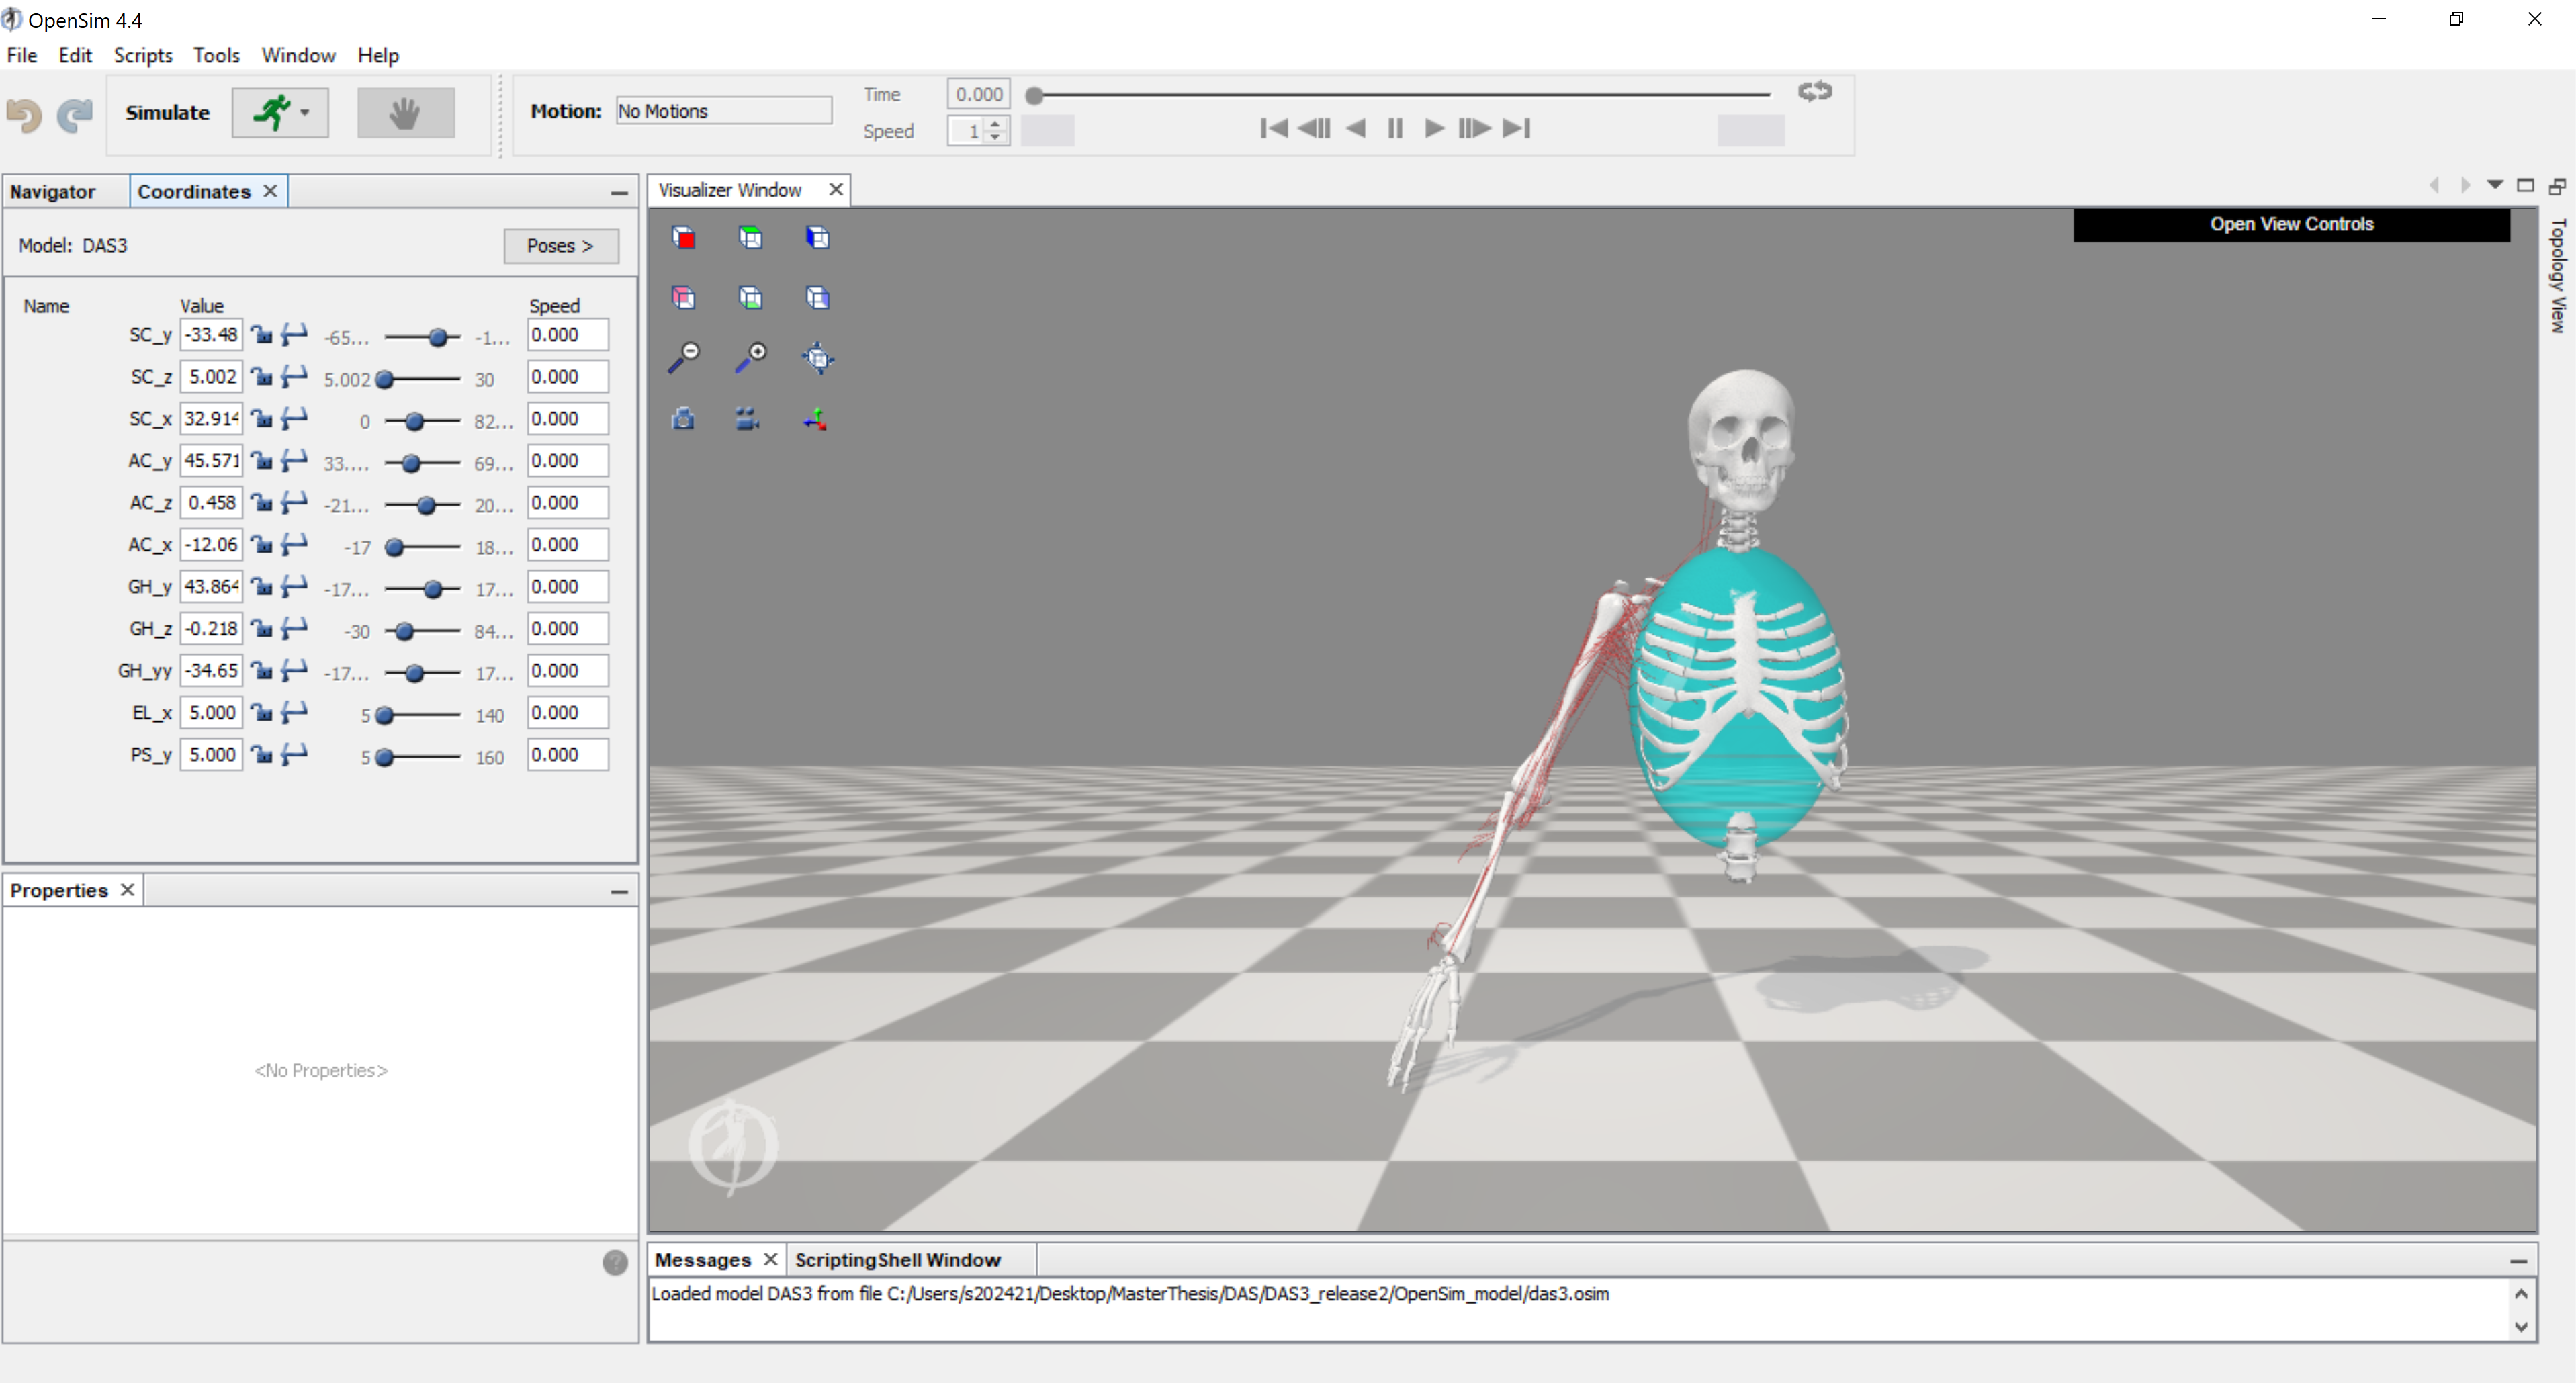
\includegraphics[width=0.7\textwidth]{Pictures/OpenSimModel.png}
    \caption{Open Sim DAS}
    \label{fig:OpenSimDAS}
\end{figure}

\begin{lstlisting}
    d = das3('Visualization',x);   
    p = d(j,1:3)';					% position vector of bone
	R = reshape(d(j,4:12),3,3)';	% orientation matrix
 \end{lstlisting}


Use cases and practical examples.

\subsubsection{Dynamics of DAS}
\subsubsection{Joint Moments}
\subsubsection{Stick}

\section{Conclusion}